\documentclass{beamer}
\usepackage[english,greek]{babel}
\usepackage[iso-8859-7]{inputenc}
\usepackage{amsthm,amsmath,amssymb,graphicx,bbm,extarrows,float,tikz,changepage,subcaption,ifthen,chngcntr,soul,setspace,parskip,cancel}
\usepackage{hyperref}
\usetikzlibrary{decorations.pathreplacing}
\usetikzlibrary{decorations.pathmorphing}
\usetikzlibrary{arrows.meta}
\usetikzlibrary{arrows}
\usetikzlibrary{positioning,matrix,scopes,fit,svg.path}
\usetikzlibrary{patterns}
\usetikzlibrary{intersections}
\usetikzlibrary{calc}
%\usetheme{CambridgeUS}
%\usecolortheme{orchid}

\beamertemplatenavigationsymbolsempty

\uselanguage{greek}

\setbeamertemplate{itemize items}[default]
  
\newcommand{\R}{\mathbb{R}}

\pgfdeclarelayer{bg}
\pgfsetlayers{bg,main}

\let\sin\relax
\DeclareMathOperator{\sin}{\text{��}}

\let\cos\relax
\DeclareMathOperator{\cos}{\text{���}}

\let\tan\relax
\DeclareMathOperator{\tan}{\text{��}}

\begin{document}
\begin{frame}[plain]
\begin{figure}[!htb]
\centering
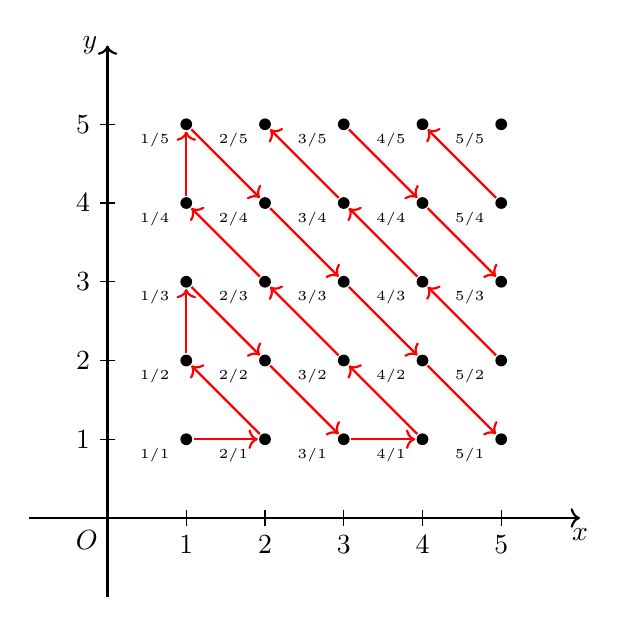
\begin{tikzpicture}
\draw[thick,->,name path=x axis] (-1,0) -- (6,0)node[pos=1,below]{$x$};
\draw[thick,->,name path=y axis] (0,-1) -- (0,6)node[pos=1,left]{$y$};
\node[left,yshift=-8pt](O) at (0,0){$O$};
\foreach \i in {1,...,5}{
    \draw (\i,-.1) -- (\i,.1)node[pos=0,below]{\i};
    \draw (.1,\i) -- (-.1,\i)node[pos=1,left]{\i};
    \foreach \j in {1,...,5}{
        \node[circle, fill=black, inner sep=1.5pt, outer sep=.5pt, label={left,yshift=-.2cm}:{$\scriptscriptstyle\i/\j$}](\i\j) at (\i,\j){};
    }
}
\draw[thick,red,->] (11) -- (21);
\draw[thick,red,->] (21) -- (12);
\draw[thick,red,->] (12) -- (13);
\draw[thick,red,->] (13) -- (22);
\draw[thick,red,->] (22) -- (31);
\draw[thick,red,->] (31) -- (41);
\draw[thick,red,->] (41) -- (32);
\draw[thick,red,->] (32) -- (23);
\draw[thick,red,->] (23) -- (14);
\draw[thick,red,->] (14) -- (15);
\draw[thick,red,->] (15) -- (24);
\draw[thick,red,->] (24) -- (33);
\draw[thick,red,->] (33) -- (42);
\draw[thick,red,->] (42) -- (51);
\draw[thick,red,->] (52) -- (43);
\draw[thick,red,->] (43) -- (34);
\draw[thick,red,->] (34) -- (25);
\draw[thick,red,->] (35) -- (44);
\draw[thick,red,->] (44) -- (53);
\draw[thick,red,->] (54) -- (45);
\end{tikzpicture}
\end{figure}
\end{frame}
\end{document}